\chapter{Introducción}

En este primer capítulo se expone el contexto y motivación del proyecto, los objetivos planteados, la planificación y costes, y por último la estructura que se seguirá en la memoria.

\section{Contexto y motivación}

La transformación digital del sector sanitario ha avanzado de forma decidida en las últimas décadas. En Estados Unidos, por ejemplo, cerca del 96\% de los hospitales ya habían adoptado sistemas de historiales clínicos electrónicos (EHR) para 2015 \cite{Henry2016_EHR}. Este avance ha generado un volumen masivo de datos clínicos, fundamentales para la investigación en áreas como la epidemiología o el desarrollo de modelos predictivos \cite{Halevy2009_data}. Sin embargo, aunque la generación de datos es continua y creciente, la mayoría de estos registros están sujetos a estrictas restricciones de acceso debido a cuestiones legales, éticas y, sobre todo, de privacidad del paciente. Esta protección, imprescindible para salvaguardar la confidencialidad, limita el potencial de los datos para la investigación y la innovación clínica.

En este contexto, la aparición de bases de datos como MIMIC-III \cite{MIMICIII_paper} (Medical Information Mart for Intensive Care) supuso un hito al demostrar que es posible compartir datos clínicos reales de forma segura mediante procesos rigurosos de desidentificación, permitiendo así la realización de cientos de estudios que han mejorado la práctica clínica \cite{Kallout2025_contribution}. El proyecto MIMIC-IV \cite{MIMICIV_paper, MIMICIV_dataset}, sobre el que se fundamenta este trabajo, continúa y amplía ese legado con información clínica detallada y anonimizada del Beth Israel Deaconess Medical Center de Boston. En su versión 3.1, MIMIC-IV incluye datos de más de 364.000 pacientes y casi 550.000 admisiones hospitalarias, abarcando desde datos demográficos y resultados de laboratorio hasta procedimientos médicos y evolución clínica.

\newpage
No obstante, a pesar de la riqueza y el potencial de MIMIC-IV, persiste un reto relevante: extraer conocimiento útil de estos datos sigue siendo complejo para quienes no poseen formación técnica avanzada. La barrera tecnológica impide que muchos profesionales sanitarios, investigadores clínicos y estudiantes puedan aprovechar plenamente la información disponible~\cite{Khaled2025,AlAttrach2025}. Ante esta situación, la motivación fundamental de este proyecto es precisamente derribar ese obstáculo, desarrollando una plataforma donde cualquier usuario pueda visualizar, explorar y descubrir patrones complejos en los datos, acelerando así la generación de hipótesis y la toma de decisiones fundamentadas en evidencia real.


\section{Objetivos}

\subsection{Objetivo general}

Este proyecto tiene como objetivo principal desarrollar una aplicación web con Inteligencia Artificial que permita visualizar, analizar, predecir y explicar historiales clínicos contenidos en MIMIC-IV.

\subsection{Objetivos específicos}

\begin{itemize}
\item \textbf{OE1.} Investigar sobre el problema y sus posibles soluciones.
\item \textbf{OE2.} Almacenar el conjunto de datos MIMIC-IV en una base de datos para poder realizar consultas eficientes.
\item \textbf{OE3.} Desarrollar un backend API RESTful que sirva como intermediario entre la base de datos y el frontend.
\item \textbf{OE4.} Construir una plataforma web con interfaz intuitiva y visualizaciones dinámicas para facilitar la interpretación de los datos.
\item \textbf{OE5.} Implementar funcionalidades con IA que permita realizar consultas en lenguaje natural sobre la base de datos y obtener resumenes del historial de un paciente.
\item \textbf{OE6.} Configurar el entorno de producción para el acceso público de la herramienta.
\item \textbf{OE7.} Redacción de la memoria.
\end{itemize}

\newpage
\section{Planificación}

En esta sección se presenta un diagrama de Gantt que recoge la planificación temporal del proyecto, abarcando los meses de marzo a agosto. El diagrama refleja las principales tareas a realizar, correspondientes a los siete objetivos específicos expuestos previamente, y permite visualizar la distribución y el solapamiento de actividades a lo largo de todo el desarrollo.

\begin{figure}[H]
    \centering
    \fbox{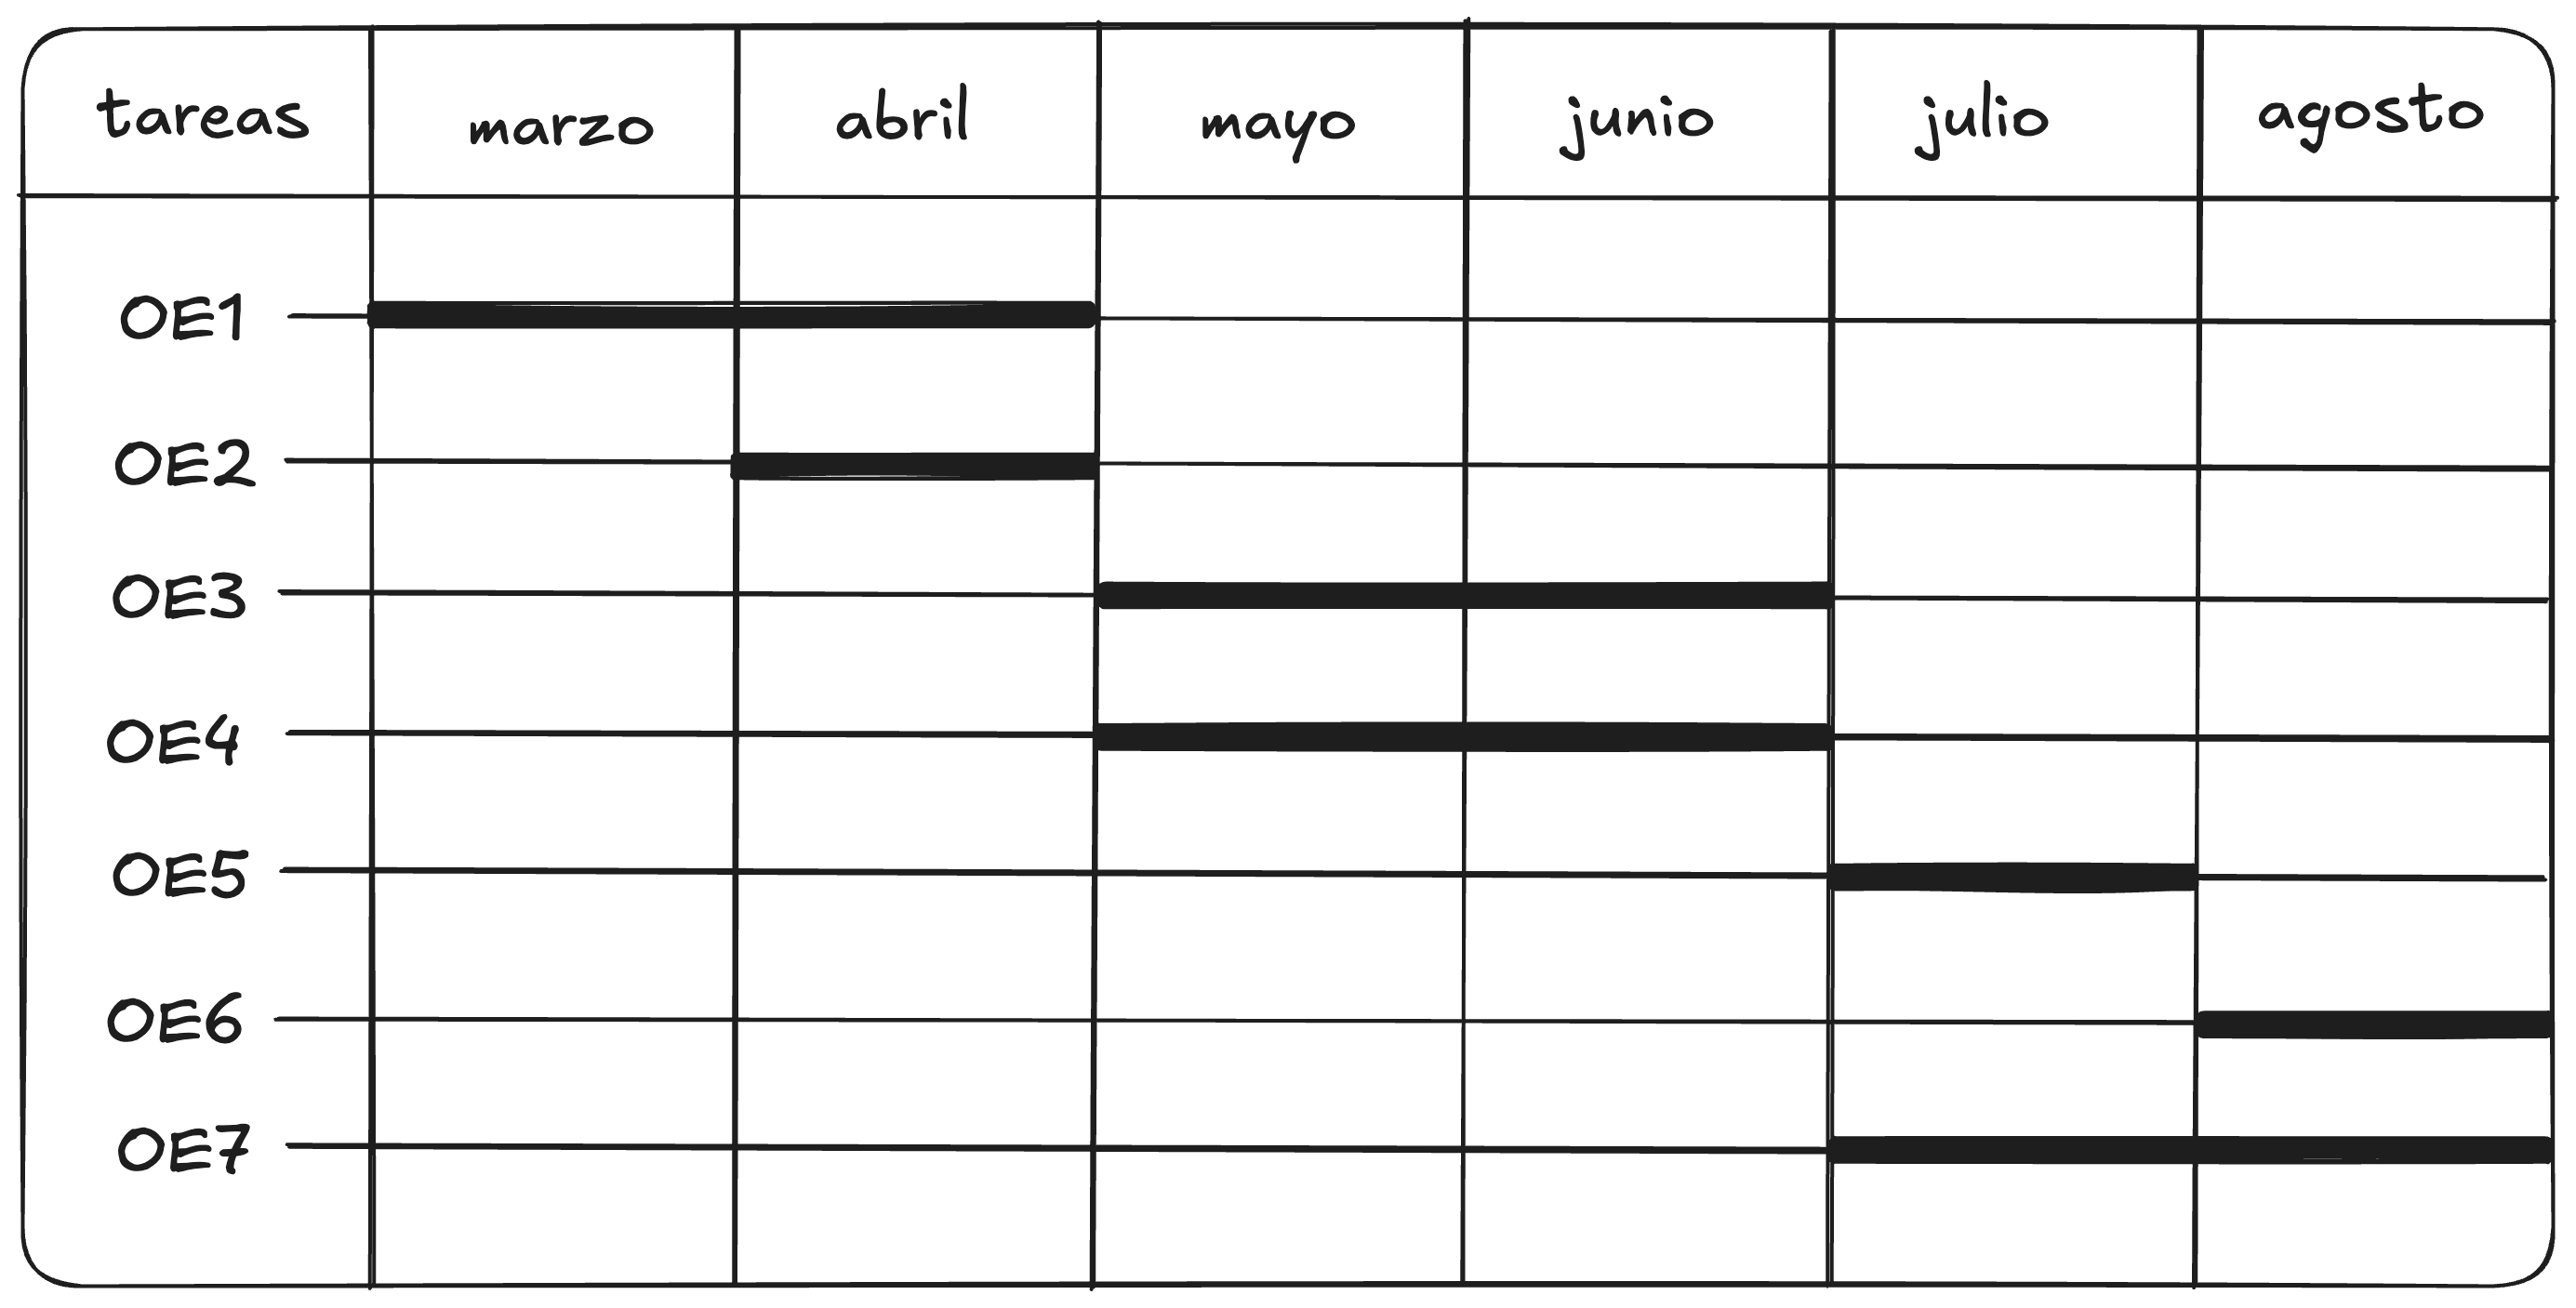
\includegraphics[width=\textwidth]{imagenes/gantt1.png}}
    %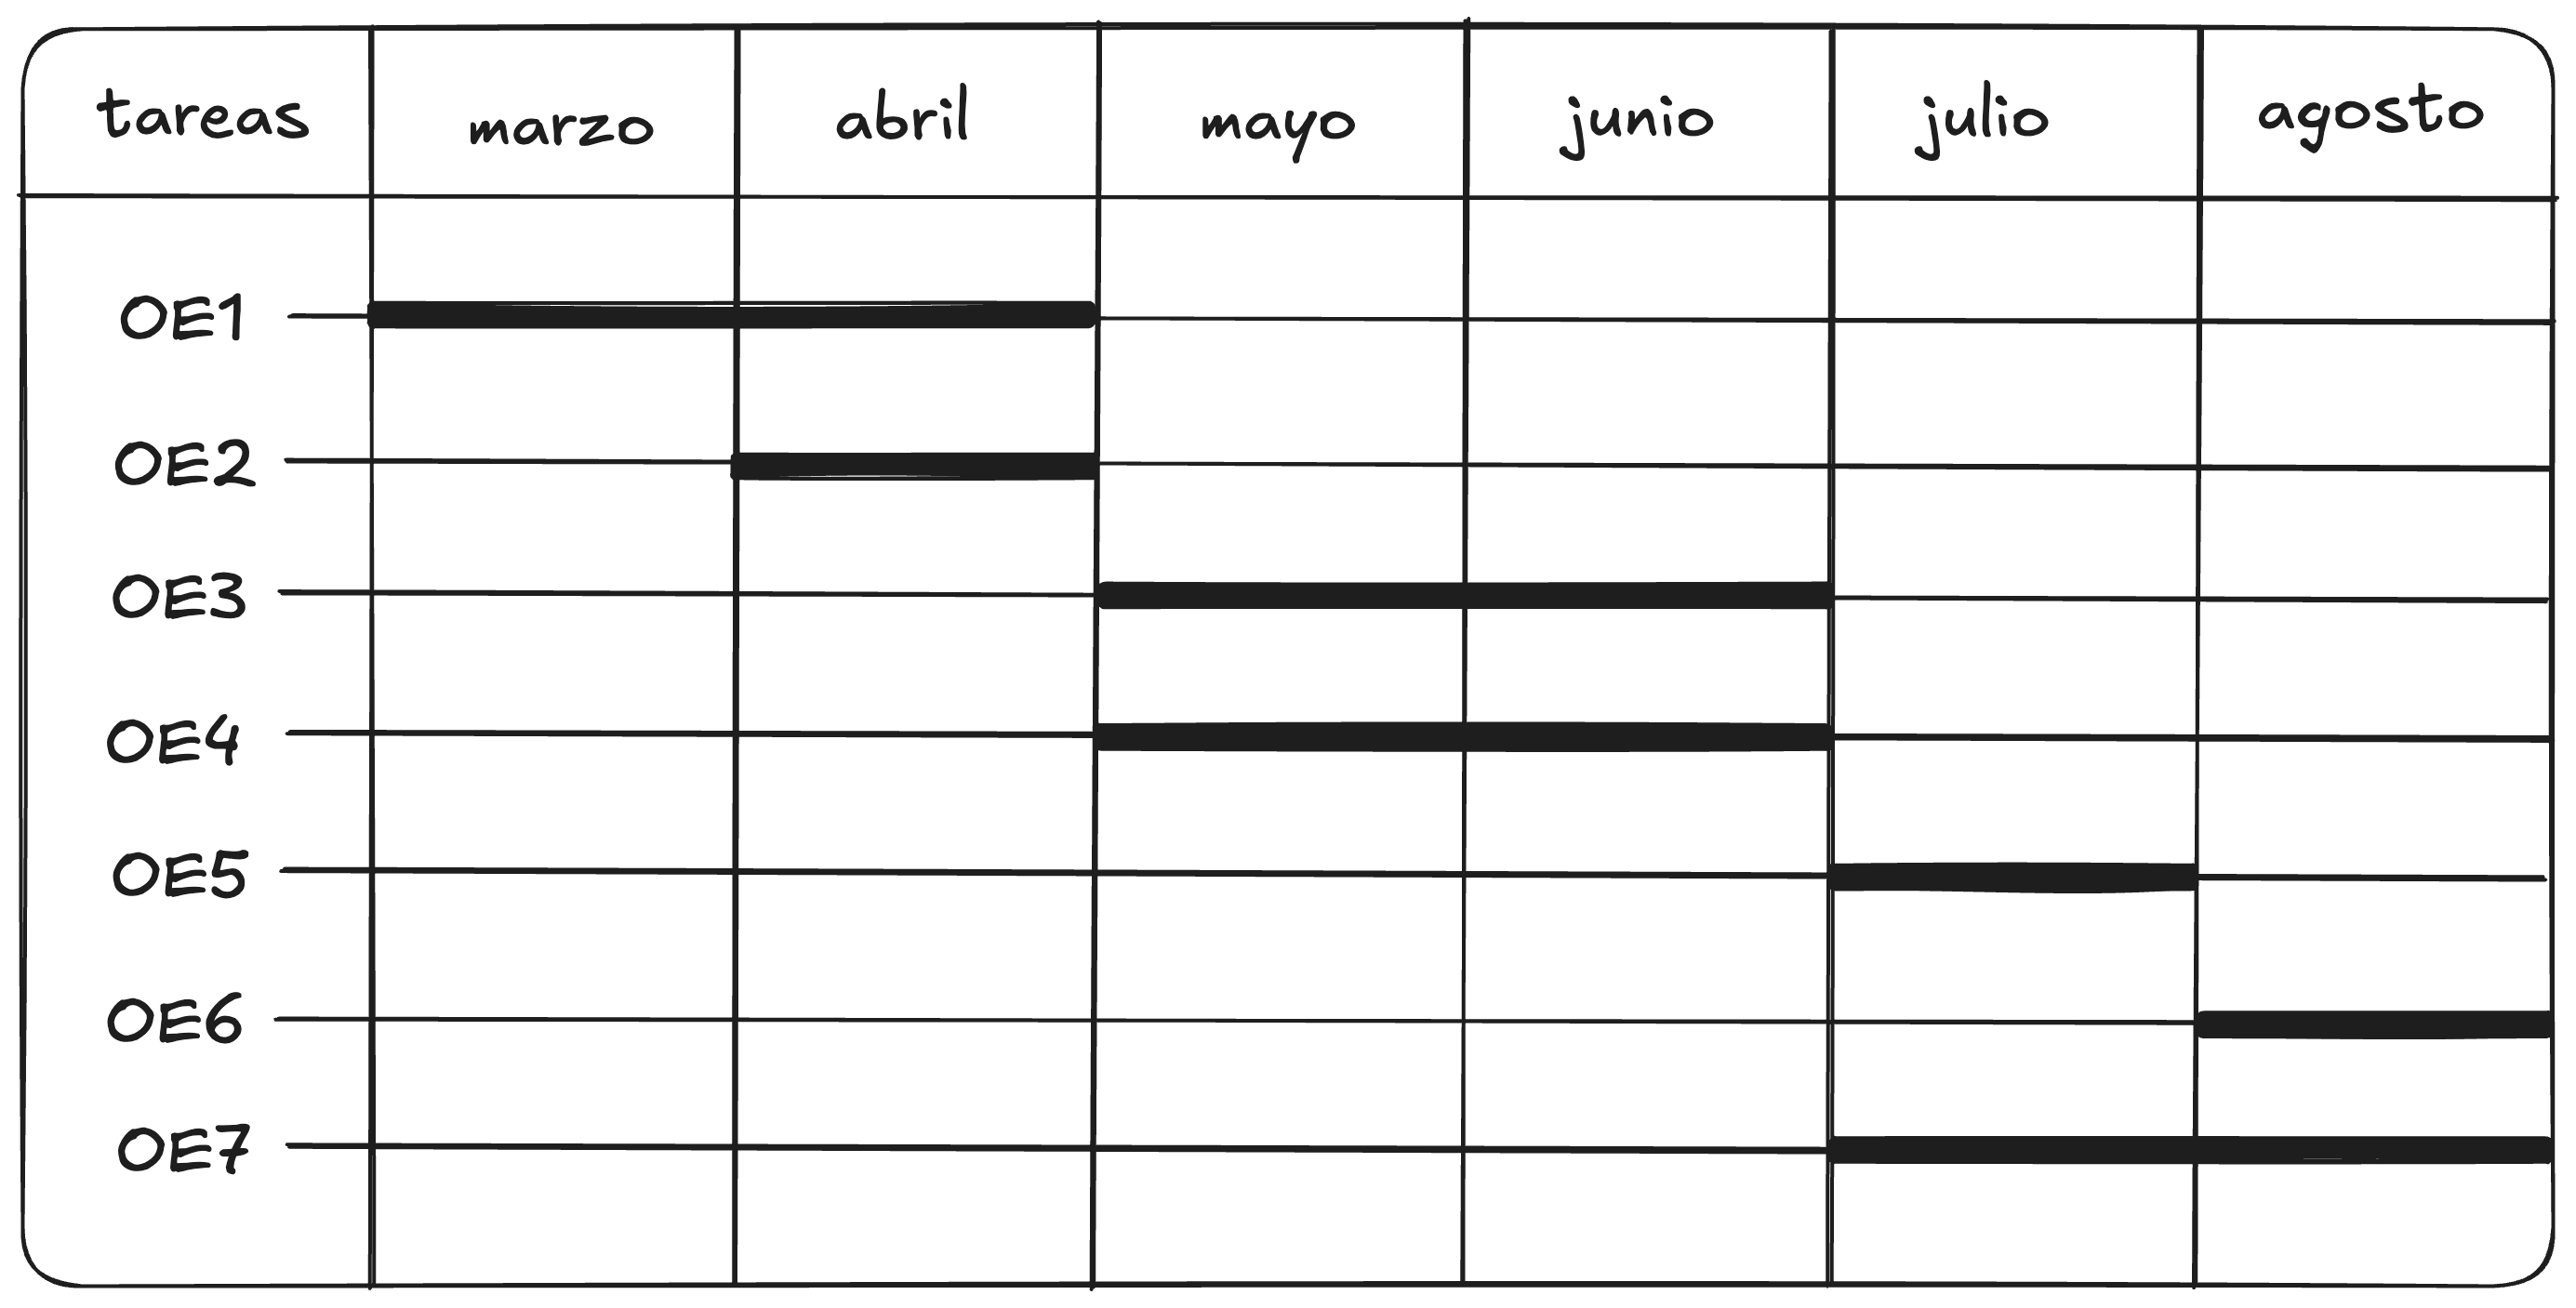
\includegraphics[width=\textwidth]{imagenes/gantt1.png}
    \caption{Diagrama de Gantt con la planificación del proyecto.}
\end{figure}

\section{Costes}

Si bien este proyecto tiene un enfoque académico, la elaboración de un presupuesto permite obtener una perspectiva más objetiva sobre el trabajo realizado. Este ejercicio aporta tanto un marco técnico como económico, acercando la iniciativa a escenarios reales y facilitando estimaciones útiles para futuras implementaciones o propuestas. Asimismo, contribuye a fundamentar las decisiones técnicas en función de su viabilidad financiera.

Para la estimación de costes, se han tenido en cuenta los recursos humanos, el equipamiento tecnológico y las herramientas de software empleadas. El cálculo se apoya en las tarifas promedio del sector de la programación en España y en los recursos técnicos requeridos. Los datos salariales se han extraído de la plataforma Glassdoor \cite{glassdoor}. Se ha considerado una duración total del proyecto de cinco meses.

\subsubsection{Costes humanos}

Para simular el coste de desarrollo de la plataforma en un entorno real, se ha considerado la contratación de un desarrollador junior a jornada completa (8 horas diarias, 21 días laborables al mes), lo que supone 168 horas mensuales. El salario anual medio para este perfil en España se estima en 20.000€.

\begin{equation*}
\text{Horas trabajadas al año} = 168\,\text{horas/mes} \times 12\,\text{meses} = 2.016\,\text{horas/año}
\end{equation*}

\begin{equation*}
\text{Coste por hora} = \frac{20.000\,€}{2.016\,\text{horas}} \approx 9,92\,€/hora
\end{equation*}

\begin{equation*}
\text{Coste mensual} = 9,92\,€/hora \times 168\,\text{horas} = 1.666,56\,€
\end{equation*}

\begin{equation*}
\text{Coste total (5 meses)} = 1.666,56\,€ \times 5 = 8.332,80\,€
\end{equation*}

\subsubsection{Costes de material}

Para el desarrollo del proyecto se han utilizado los siguientes equipos:

\begin{center}
\begin{tabular}{|l|c|}
\hline
\textbf{Material} & \textbf{Coste (€)} \\
\hline
Ordenador portátil & 2.000 \\
Servidor doméstico & 500 \\
\hline
\textbf{Total} & \textbf{2.500} \\
\hline
\end{tabular}
\end{center}

\subsubsection{Costes de herramientas}

Todo el software empleado en el desarrollo del proyecto corresponde a herramientas de licencia gratuita o planes gratuitos, por lo que no suponen coste adicional. No obstante, se ha utilizado la API de OpenAI con un coste total de 20€, además de un dominio personalizado con coste de 10€.

\begin{center}
\begin{tabular}{|l|c|}
\hline
\textbf{Herramienta} & \textbf{Coste (€)} \\
\hline
Software (licencias gratuitas) & 0 \\
Dominio & 10 \\
API OpenAI & 20 \\
\hline
\textbf{Total} & \textbf{30} \\
\hline
\end{tabular}
\end{center}

\subsubsection{Resumen de costes}

A continuación se muestra un resumen de todos los costes estimados para el proyecto:

\begin{center}
\begin{tabular}{|l|c|}
\hline
\textbf{Concepto} & \textbf{Coste (€)} \\
\hline
Coste de personal & 8.332,80 \\
Coste de material & 2.500 \\
Coste de herramientas & 30 \\
\hline
\textbf{Total} & \textbf{10.862,80} \\
\hline
\end{tabular}
\end{center}
\section{Estructura de la memoria}

El presente documento se estructura de la siguiente manera:

\begin{itemize}
    \item \textbf{Capítulo 1: Introducción}. Presenta el contexto, motivación, objetivos del proyecto, su planificación y costes, y finalmente la estructura de la memoria.
    
    \item \textbf{Capítulo 2: Estado del arte}. Revisión profunda de la literatura y trabajos previos.

    
    %\item \textbf{Capítulo 3: Diseño}. Descripción detallada de la arquitectura, modelos de datos y diseño de interfaces de la aplicación.
    
    \item \textbf{Capítulo 3: Implementación}. Explicación detallada de todos los componentes de la solución implementada.
    
    %\item \textbf{Capítulo 5: Resultados y evaluación}. Presentación de los resultados obtenidos y evaluación del desempeño de la aplicación en términos de usabilidad, eficiencia y utilidad.
    
    \item \textbf{Capítulo 4: Conclusiones y trabajo futuro}. Resumen de las contribuciones del proyecto y posibles líneas de trabajo futuro.
\end{itemize}
